%Input preamble
%Style
\documentclass[12pt]{article}
\usepackage[top=1in, bottom=1in, left=1in, right=1in]{geometry}
\parindent 22pt
\usepackage{fancyhdr}

%Packages
\usepackage{adjustbox}
\usepackage{amsmath}
\usepackage{amsfonts}
\usepackage{amssymb}
\usepackage{bm}
\usepackage[table]{xcolor}
\usepackage{tabu}
\usepackage{color,soul}
\usepackage{makecell}
\usepackage{longtable}
\usepackage{multirow}
\usepackage[normalem]{ulem}
\usepackage{etoolbox}
\usepackage{graphicx}
\usepackage{tabularx}
\usepackage{ragged2e}
\usepackage{booktabs}
\usepackage{caption}
\usepackage{fixltx2e}
\usepackage[para, flushleft]{threeparttablex}
\usepackage[capposition=top,objectset=centering]{floatrow}
\usepackage{subcaption}
\usepackage{pdfpages}
\usepackage{pdflscape}
\usepackage{natbib}
\usepackage{bibunits}
\definecolor{maroon}{HTML}{990012}
\usepackage[colorlinks=true,linkcolor=maroon,citecolor=maroon,urlcolor=maroon,anchorcolor=maroon]{hyperref}
\usepackage{marvosym}
\usepackage{makeidx}
\usepackage{tikz}
\usetikzlibrary{shapes}
\usepackage{setspace}
\usepackage{enumerate}
\usepackage{rotating}
\usepackage{tocloft}
\usepackage{epstopdf}
\usepackage[titletoc]{appendix}
\usepackage{framed}
\usepackage{comment}
\usepackage{xr}
\usepackage{titlesec}
\usepackage{footnote}
\usepackage{longtable}
\newlength{\tablewidth}
\setlength{\tablewidth}{9.3in}
\setcounter{secnumdepth}{4}

\titleformat{\paragraph}
{\normalfont\normalsize\bfseries}{\theparagraph}{1em}{}
\titlespacing*{\paragraph}
{0pt}{3.25ex plus 1ex minus .2ex}{1.5ex plus .2ex}
\makeatletter
\pretocmd\start@align
{%
  \let\everycr\CT@everycr
  \CT@start
}{}{}
\apptocmd{\endalign}{\CT@end}{}{}
\makeatother
%Watermark
\usepackage[printwatermark]{xwatermark}
\usepackage{lipsum}
\definecolor{lightgray}{RGB}{220,220,220}
%\newwatermark[allpages,color=lightgray,angle=45,scale=3,xpos=0,ypos=0]{Preliminary Draft}

%Further subsection level
\usepackage{titlesec}
\setcounter{secnumdepth}{4}
\titleformat{\paragraph}
{\normalfont\normalsize\bfseries}{\theparagraph}{1em}{}
\titlespacing*{\paragraph}
{0pt}{3.25ex plus 1ex minus .2ex}{1.5ex plus .2ex}

\setcounter{secnumdepth}{5}
\titleformat{\subparagraph}
{\normalfont\normalsize\bfseries}{\thesubparagraph}{1em}{}
\titlespacing*{\subparagraph}
{0pt}{3.25ex plus 1ex minus .2ex}{1.5ex plus .2ex}

%Functions
\DeclareMathOperator{\cov}{Cov}
\DeclareMathOperator{\corr}{Corr}
\DeclareMathOperator{\var}{Var}
\DeclareMathOperator{\plim}{plim}
\DeclareMathOperator*{\argmin}{arg\,min}
\DeclareMathOperator*{\argmax}{arg\,max}

%Math Environments
\newtheorem{theorem}{Theorem}
\newtheorem{claim}{Claim}
\newtheorem{condition}{Condition}
\renewcommand\thecondition{C--\arabic{condition}}
\newtheorem{algorithm}{Algorithm}
\newtheorem{assumption}{Assumption}
\renewcommand\theassumption{A--\arabic{assumption}}
\newtheorem{remark}{Remark}
\renewcommand\theremark{R--\arabic{remark}}
\newtheorem{definition}[theorem]{Definition}
\newtheorem{hypothesis}[theorem]{Hypothesis}
\newtheorem{property}[theorem]{Property}
\newtheorem{example}[theorem]{Example}
\newtheorem{result}[theorem]{Result}
\newenvironment{proof}{\textbf{Proof:}}{$\bullet$}

%Commands
\newcommand\independent{\protect\mathpalette{\protect\independenT}{\perp}}
\def\independenT#1#2{\mathrel{\rlap{$#1#2$}\mkern2mu{#1#2}}}
\newcommand{\overbar}[1]{\mkern 1.5mu\overline{\mkern-1.5mu#1\mkern-1.5mu}\mkern 1.5mu}
\newcommand{\equald}{\ensuremath{\overset{d}{=}}}
\captionsetup[table]{skip=10pt}
%\makeindex

\setlength\parindent{0pt}
\setlength{\parskip}{10pt}

\newcolumntype{L}[1]{>{\raggedright\let\newline\\\arraybackslash\hspace{0pt}}m{#1}}
\newcolumntype{C}[1]{>{\centering\let\newline\\\arraybackslash\hspace{0pt}}m{#1}}
\newcolumntype{R}[1]{>{\raggedleft\let\newline\\\arraybackslash\hspace{0pt}}m{#1}}



%Logo
%\AddToShipoutPictureBG{%
%  \AtPageUpperLeft{\raisebox{-\height}{
\includegraphics[width=1.5cm]{uchicago.png}}}
%}

\newcolumntype{L}[1]{>{\raggedright\let\newline\\\arraybackslash\hspace{0pt}}m{#1}}
\newcolumntype{C}[1]{>{\centering\let\newline\\\arraybackslash\hspace{0pt}}m{#1}}
\newcolumntype{R}[1]{>{\raggedleft\let\newline\\\arraybackslash\hspace{0pt}}m{#1}}

\newcommand{\mr}{\multirow}
\newcommand{\mc}{\multicolumn}

%\newcommand{\comment}[1]{}

%Other parameters
\newcommand{\noutcomes}{95}
\newcommand{\noutcomesexpp}{357}
\newcommand{\noutcomesexpm}{343}
\newcommand{\noutcomesexpf}{355}
\newcommand{\treatsubsabc}{$75\%$}
\newcommand{\treatsubscarec}{$74\%$}
\newcommand{\treatsubscaref}{$63\%$}

%Counts
%Males
\newcommand{\positivem}{$78\%$}
\newcommand{\positivesm}{$29\%$}

%Females
\newcommand{\positivef}{$78\%$}
\newcommand{\positivesf}{$31\%$}

%Counts, control substitution
%Males
\newcommand{\positivecsnm}{$47\%$}
\newcommand{\positivescsnm}{$15\%$}

\newcommand{\positivecsam}{$79\%$}
\newcommand{\positivescsam}{$29\%$}

%Females
%% no alternative
\newcommand{\positivecsnf}{$84\%$}
\newcommand{\positivescsnf}{$55\%$}

%% alternative
\newcommand{\positivecsaf}{$79\%$}
\newcommand{\positivescsaf}{$33\%$}

%Pooled

%Effects
%Males

%Females
\newcommand{\empf}{$8$}
\newcommand{\yearsedf}{$1.7$}



%Pooled

%CBA
%IRR
%Males
\newcommand{\irrm}{$15\%$}
\newcommand{\irrsem}{$5\%$}

%Females
\newcommand{\irrf}{$9\%$}
\newcommand{\irrsef}{$7\%$}

%Pooled
\newcommand{\irrp}{$13\%$}
\newcommand{\irrsep}{$5\%$}

%BC
%Males
\newcommand{\bcm}{$11.24$}
\newcommand{\bcsem}{$4.60$}

%Females
\newcommand{\bcf}{$2.35$}
\newcommand{\bcsef}{$1.09$}

%Pooled
\newcommand{\bcp}{$5.63$}
\newcommand{\bcsep}{$2.15$}

%NPV streams
%Pooled
\newcommand{\parincomenpvp}{$\$119,346$}

\usepackage[stable]{footmisc}

\newcommand*\leftright[2]{%
  \leavevmode
  \rlap{#1}%
  \hspace{0.5\linewidth}%
  #2}

\newcommand{\orth}{\ensuremath{\perp\!\!\!\perp}}%
\newcommand{\indep}{\orth}%
\newcommand{\notorth}{\ensuremath{\perp\!\!\!\!\!\!\diagup\!\!\!\!\!\!\perp}}%
\newcommand{\notindep}{\notorth}


\begin{document}

\begin{titlepage}
\newgeometry{top=.8in, bottom=.8in, left=.8in, right=.8in}

\title{\Large \textbf{Gender Differences in the Benefits of a Prototypical Early Childhood Program: \\ Large Graphs of Gender Gaps}}

\author{
Jorge Luis Garc\'{i}a\\
Department of Economics\\
The University of Chicago \and
James J. Heckman \\
American Bar Foundation \\
Department of Economics\\
The University of Chicago \and
Anna L. Ziff \\
Center for the Economics of \\
Human Development \\
The University of Chicago}
\date{First Draft: January 5, 2016\\ This Draft: \today}

\maketitle

\textbf{[We replaced the main plots with tables. We think they more clearly show the accounting exercise by explicitly listing the difference between the proportions of the treatment and control groups.]}

\restoregeometry
\end{titlepage}

\begin{table}[H]
\centering
\caption{Summary of Proportion of Outcomes Males $>$ Females}
\label{tab:proportion-table}
\begin{threeparttable}
\begin{tabular}{l c c c c}
\toprule
Category & \# Outcomes & \mc{2}{c}{Proportion} & Difference \\
\cmidrule(lr){3-4} \cmidrule(lr){5-5}
            &                       & Control & Treatment & Treatment $- $ Control \\
\midrule
IQ & 15 & 0.733 & 0.533 & -0.200 \\
Achievement & 12 & \textbf{0.833} & \textbf{0.000} & \textbf{-0.833} \\
Social-emotional & 22 & 0.455 & 0.364 & \textbf{-0.091} \\
Parenting & 7 & 0.571 & 0.286 & \textbf{-0.286} \\
Parental Income & 15 & 0.600 & 0.733 & 0.133 \\
Education & 9 & 0.667 & \textbf{0.111} & \textbf{-0.556} \\
Employment & 4 & \textbf{1.000} & \textbf{0.750} & \textbf{-0.250} \\
Crime & 4 & \textbf{0.000} & \textbf{0.000} & \textbf{0.000} \\
Risky Behavior & 5 & 0.400 & \textbf{0.200} & \textbf{-0.200} \\
Health & 22 & 0.500 & \textbf{0.682} & \textbf{0.182} \\
Mental Health & 11 & \textbf{0.818} & 0.545 & \textbf{-0.273} \\
\midrule
All & 126 & 0.603 & 0.437 & \textbf{-0.167} \\
\bottomrule
\end{tabular}
% This file generated by: abccare-cba/scripts/abccare/genderdifferences/abccare-gdiff-gaps-ranksign.do

\begin{tablenotes}
\footnotesize
\item Note: This table summarizes comparison of gender gaps across outcome categories by different groups. A bold proportion for the treatment or control group indicates that the proportion is statistically different than 50\%. A bold difference between treatment and control indicates that the rank sign test over 100 bootstraps yields a $p$-value less than or equal to 0.10. 
\end{tablenotes}
\end{threeparttable}
\end{table}

\begin{table}[H]
\centering
\caption{Summary of Proportion of Outcomes Males $>$ Females, Stay at Home}
\label{tab:proportion-table}
\begin{threeparttable}
\begin{tabular}{l c c c c}
\toprule
Category & \# Outcomes & \mc{2}{c}{Proportion} & Difference \\
\cmidrule(lr){3-4} \cmidrule(lr){5-5}
            &                       & Control & Treatment & Treatment $- $ Control \\
\midrule
IQ & 15 & \textbf{1.000} & 0.533 & \textbf{-0.467} \\
Achievement & 12 & \textbf{1.000} & \textbf{0.000} & \textbf{-1.000} \\
Social-Emotional & 22 & 0.591 & \textbf{0.364} & \textbf{-0.227} \\
Parenting & 7 & \textbf{1.000} & 0.286 & \textbf{-0.714} \\
Parental Labor Income & 15 & \textbf{0.800} & 0.733 & \textbf{-0.067} \\
Education & 9 & \textbf{0.667} & \textbf{0.111} & \textbf{-0.556} \\
Employment & 4 & \textbf{1.000} & \textbf{0.750} & \textbf{-0.250} \\
Crime & 4 & 0.500 & \textbf{0.000} & \textbf{-0.500} \\
Risky Behavior & 5 & \textbf{0.200} & \textbf{0.200} & \textbf{0.000} \\
Health & 22 & 0.545 & 0.545 & 0.000 \\
Mental Health & 11 & \textbf{1.000} & 0.545 & \textbf{-0.455} \\
\midrule
All & 126 & \textbf{0.754} & 0.413 & \textbf{-0.341} \\
\bottomrule
\end{tabular}
% This file generated by: abccare-cba/scripts/abccare/genderdifferences/abccare-gdiff-gaps-ranksign.do

\begin{tablenotes}
\footnotesize
\item Note: This table summarizes comparison of gender gaps across outcome categories by different groups. A bold proportion for the treatment or control group indicates that the proportion is statistically different than 50\%. A bold difference between treatment and control indicates that the rank sign test over 100 bootstraps yields a $p$-value less than or equal to 0.10. 
\end{tablenotes}
\end{threeparttable}
\end{table}

\begin{table}[H]
\centering
\caption{Summary of Proportion of Outcomes Males $>$ Females, Alternative Preschool}
\label{tab:proportion-table}
\begin{threeparttable}
\begin{tabular}{l c c c c}
\toprule
Category & \# Outcomes & \mc{2}{c}{Proportion} & Difference \\
\cmidrule(lr){3-4} \cmidrule(lr){5-5}
            &                       & Control & Treatment & Treatment $- $ Control \\
\midrule
IQ & 15 & 0.267 & 0.533 & \textbf{0.267} \\
Achievement & 12 & 0.250 & \textbf{0.000} & \textbf{-0.250} \\
Social-emotional & 22 & \textbf{0.318} & \textbf{0.364} & \textbf{0.045} \\
Parenting & 7 & 0.429 & 0.286 & -0.143 \\
Parental Income & 15 & 0.467 & 0.733 & \textbf{0.267} \\
Education & 9 & 0.444 & \textbf{0.111} & \textbf{-0.333} \\
Employment & 4 & 0.500 & \textbf{0.750} & \textbf{0.250} \\
Crime & 4 & \textbf{0.000} & \textbf{0.000} & \textbf{0.000} \\
Risky Behavior & 5 & 0.600 & \textbf{0.200} & \textbf{-0.400} \\
Health & 22 & 0.500 & 0.545 & \textbf{0.045} \\
Mental Health & 11 & 0.545 & 0.545 & \textbf{0.000} \\
\midrule
All & 126 & 0.397 & 0.413 & \textbf{0.016} \\
\bottomrule
\end{tabular}
% This file generated by: abccare-cba/scripts/abccare/genderdifferences/abccare-gdiff-gaps-ranksign.do

\begin{tablenotes}
\footnotesize
\item Note: This table summarizes comparison of gender gaps across outcome categories by different groups. A bold proportion for the treatment or control group indicates that the proportion is statistically different than 50\%. A bold difference between treatment and control indicates that the rank sign test over 100 bootstraps yields a $p$-value less than or equal to 0.10. 
\end{tablenotes}
\end{threeparttable}
\end{table}


\begin{sidewaysfigure}[H]
\centering
\caption{Proportion of Outcomes Males $>$ Females, Control Group Divided by Home Status}\label{fig3}
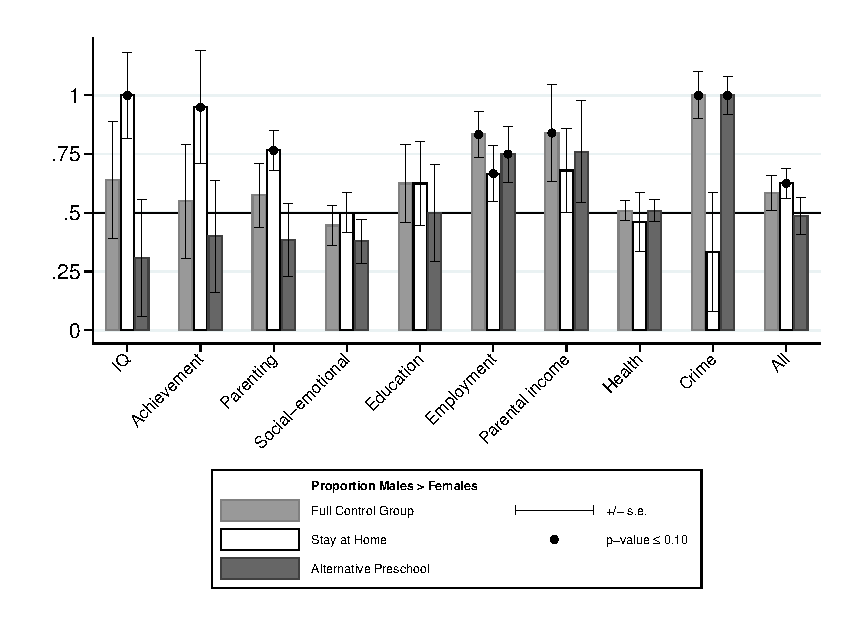
\includegraphics[width=\textwidth]{output/gendergaps-control-moderated-altpre}
\end{sidewaysfigure}

\begin{sidewaysfigure}[H]
\centering
\caption{Proportion of Outcomes Males $>$ Females, Control Group Divided by Father Present}
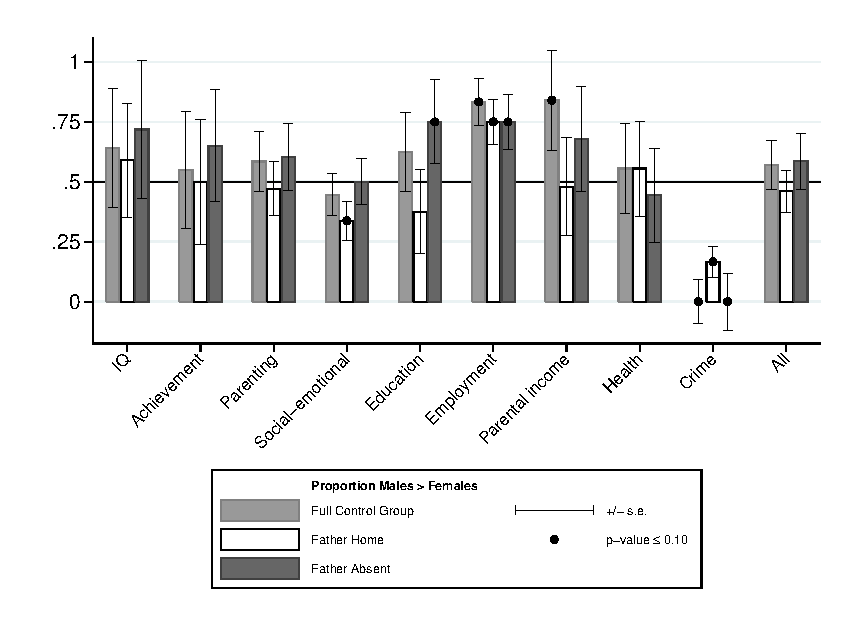
\includegraphics[width=\textwidth]{output/gendergaps-control-moderated-fhome}
\end{sidewaysfigure}

\begin{sidewaysfigure}[H]
\centering
\caption{Proportion of Outcomes Males $>$ Females, Treatment Group Divided by Father Present}
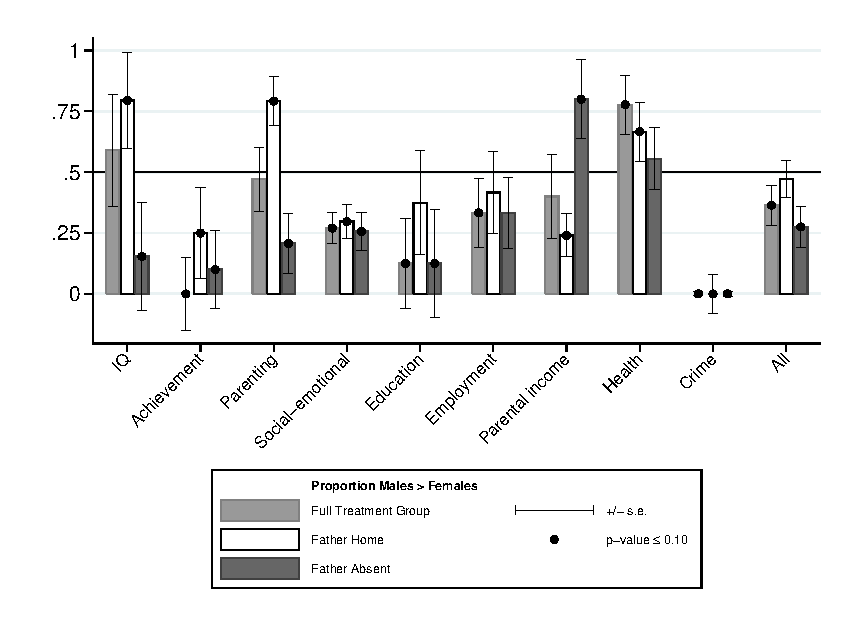
\includegraphics[width=\textwidth]{output/gendergaps-treatment-moderated-fhome}
\end{sidewaysfigure}

\begin{sidewaysfigure}[H]
\centering
\caption{Proportion of Outcomes Males $>$ Females, Control Group Divided by Mother's Locus of Control}
\label{mlocus}
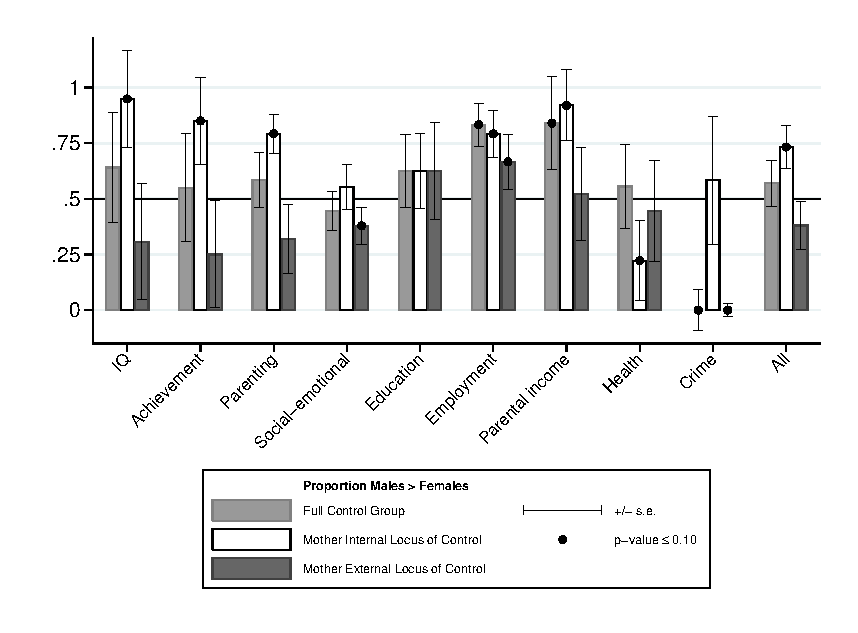
\includegraphics[width=\textwidth]{output/gendergaps-control-moderated-mlocus}
\end{sidewaysfigure}

\begin{sidewaysfigure}[H]
\centering
\caption{Proportion of Outcomes Males $>$ Females, Treatment Group Divided by Mother's Locus of Control}
\label{mlocus}
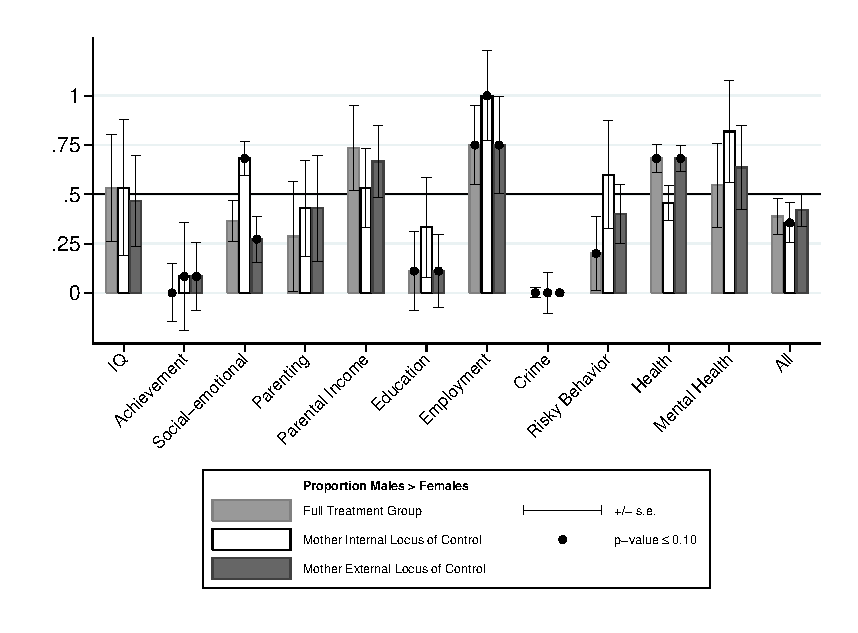
\includegraphics[width=\textwidth]{output/gendergaps-treatment-moderated-mlocus}
\end{sidewaysfigure}



\end{document}